\documentclass{article}
\usepackage[utf8]{inputenc}
\usepackage{geometry}
\usepackage[T1]{fontenc}
\usepackage{amsfonts}
\usepackage{amsmath}
\usepackage{amssymb}
\usepackage{graphicx}
\usepackage{float}
\usepackage{hyperref}
\usepackage[sorting=none]{biblatex}
\usepackage{fancyhdr}
\usepackage{multicol}
\usepackage{enumitem}
\usepackage{tikz}
\usepackage{bm}
\usetikzlibrary{shapes,arrows,fit,positioning}
\addbibresource{ref.bib}
\setlength{\columnsep}{40pt}
\setlength{\voffset}{0.7cm}
\setlength{\headsep}{40pt}
\geometry{legalpaper, portrait, margin=2cm}


% Title page
\title{HW A2\\\Large{Machine Learning, Advanced Course/DD2434/mladv24}}
\author{Andrea Stanziale \\ KTH Royal Institute of Technology}
\date{\today}

% Header and footer
\pagestyle{fancy}
\fancyhead{}
\fancyhead[L]{\textbf{Machine Learning, Advanced Course}\\\textbf{DD2434}}
\fancyhead[R]{\textbf{Andrea Stanziale}\\ stanz@kth.se}
\fancyfoot{}
\begin{document}

\maketitle

% Begin page numbers
\fancyfoot[C]{\thepage}
\pagenumbering{arabic}
\section*{Exercise 1}
\subsection*{1.1: Bayesian Network}

\begin{tikzpicture}[>=stealth, node distance=1.5cm,
  latent/.style={circle, draw, thick, minimum size=7mm, inner sep=0pt},
  observed/.style={circle, draw, thick, fill=gray!20, minimum size=7mm, inner sep=0pt},
  plate/.style={rectangle, draw, thick, inner sep=6pt, rounded corners=4pt},
  diamondnode/.style={draw, thick, shape=diamond, minimum size=8mm, inner sep=0pt},
  auto
]

  % -- Global/Hyperparameter nodes --
  \node[latent] (alpha1) at (0,3) {$\alpha^1$};
  \node[latent, below=of alpha1] (pi1) {$\pi^1$};
  \draw[->] (alpha1) -- (pi1);

  \node[latent] (alpha2) at (2,3) {$\alpha^2$};
  \node[latent, below=of alpha2] (pi2) {$\pi^2$};
  \draw[->] (alpha2) -- (pi2);

  \node[latent] (beta)  at (6,3) {$\beta_k$};
  \node[latent, below=of beta]  (rho) {$\rho_k$};
  \draw[->] (beta) -- (rho);

  % -- Per-data variables (Z^1_n, Z^2_n, then X_{n j}) --
  \node[latent]   (Z1) at (0,-1)   {$Z^1_n$};
  \node[latent]   (Z2) at (2,-1)   {$Z^2_n$};

  \node[diamondnode]   (k)  at (1, -2.5)   {$k = Z^1_n +Z^2_n$};	

  \draw[->] (pi1) -- (Z1);
  \draw[->] (pi2) -- (Z2);


  \node[observed] (X)  at (1,-4.5) {$X_{nj}$};

  \draw[->] (Z1) -- (k);
  \draw[->] (Z2) -- (k);
  \draw[->] (rho) -- (X);

  \draw[->] (k) -- (X);
  \draw[->] (k) -- (rho);



  % -- Plate for j=1..J --
  \node[plate, fit=(X), inner sep=12pt] (plateJ) {};
  \node[anchor=south east, xshift=-2pt, yshift=2pt] at (plateJ.south east) {\large $J$};

  % -- Plate for n=1..N (includes Z1, Z2, and the j-plate) --
  \node[plate, fit=(Z1)(Z2)(k)(plateJ), inner sep=12pt] (plateN) {};
  \node[anchor=south east, xshift=-2pt, yshift=2pt] at (plateN.south east) {\large $N$};

  % -- Plate for K --
  \node[plate, fit=(rho), inner sep=12pt] (plateK) {};
  \node[anchor=south east, xshift=-2pt, yshift=2pt] at (plateK.south east) {\large $K$};

\end{tikzpicture}    

\subsection*{1.2: Joint Log-Probability}
We want to express the joint log‐probability
\[
\log p\bigl(X,\;Z^1,\;Z^2,\;\pi^1,\;\pi^2,\;\rho 
\;\big|\;\alpha^1,\;\alpha^2,\;\beta \bigr).
\]
By the model factorization:
\begin{equation*}
\begin{aligned}
p(X, Z^1, Z^2, \pi^1, \pi^2, \rho \mid \alpha^1, \alpha^2, \beta) = p(\pi^1 \mid \alpha^1) p(\pi^2 \mid \alpha^2) 
\prod_k p(\rho_k \mid \beta_k) 
\prod_n \Big[ p(Z_n^1 \mid \pi^1) p(Z_n^2 \mid \pi^2) 
\prod_j p(X_{nj} \mid \rho_{k=n}) \Big]
\end{aligned}
\end{equation*}
with log‐probability:
\begin{equation*}
\begin{aligned}
&\log p(X, Z^1, Z^2, \pi^1, \pi^2, \rho \mid \alpha^1, \alpha^2, \beta)  \\
&=
\log p(\pi^1) + \log p(\pi^2) + 
\sum_k \log p(\rho_k) +
\sum_n \Big[
\log p(Z_n^1 \mid \pi^1) +
\log p(Z_n^2 \mid \pi^2) +
\sum_j \log p(X_{nj} \mid \rho_k)
\Big]
\end{aligned}
\end{equation*}
So we write the log‐probability as the sum of the following terms:
\paragraph{1. Dirichlet prior terms:}
\[
  \log p(\pi^1 \mid \alpha^1)
  \;+\;
  \log p(\pi^2 \mid \alpha^2)
  \;+\;
  \sum_{k=1}^K \log p(\rho_k \mid \beta_k).
\]
\paragraph{2. Latent class variables \(Z^1_n, Z^2_n\) given \(\pi^1, \pi^2\):}

Each \(Z^1_n\) is categorical with parameter \(\pi^1\).  In indicator function notation:
\begin{equation*} 
\log p(Z^1_n \mid \pi^1)
\;=\; 
\sum_{d=1}^{D^1} 
  \mathbf{1}\{Z^1_n = d\}\,\log \pi^1_d.
\end{equation*}

Similarly,
\[
\log p(Z^2_n \mid \pi^2)
\;=\; 
\sum_{d=1}^{D^2} 
  \mathbf{1}\{Z^2_n = d\}\,\log \pi^2_d.
\]

\paragraph{3. Observations \(\bm{X_{nj}}\) given \(\bm{\rho_{k}}\) where \(k = Z^1_n + Z^2_n\):}
\[
\log p\!\bigl(X_{nj} \mid Z^1_n, Z^2_n, \rho\bigr)
\;=\;
\sum_{m=1}^{D^3}
  \mathbf{1}\{X_{nj} = m\}\,
  \log \rho_{\,Z^1_n + Z^2_n,\;m}.
\]

\noindent
Putting these all together, the full joint log‐probability is:

\[
\begin{aligned}
&\log p\bigl(X,\!Z^1,\!Z^2,\!\pi^1,\!\pi^2,\!\rho 
    \mid \alpha^1,\!\alpha^2,\!\beta \bigr) \\
&=
\underbrace{\log p(\pi^1 \mid \alpha^1)
\;+\;
\log p(\pi^2 \mid \alpha^2)
\;+\;
\sum_{k=1}^K \log p(\rho_k \mid \beta_k)}_{\text{Dirichlet priors}}
\\[6pt]
&\quad
+\;
\sum_{n=1}^N 
\Bigl[
  \underbrace{\sum_{d=1}^{D^1} \mathbf{1}\{Z^1_n = d\}\,\log \pi^1_{d}}_{\log p(Z^1_n \mid \pi^1)}
  \;+\;
  \underbrace{\sum_{d=1}^{D^2} \mathbf{1}\{Z^2_n = d\}\,\log \pi^2_{d}}_{\log p(Z^2_n \mid \pi^2)}
\\
&\qquad\qquad\quad
  + \sum_{j=1}^J
    \underbrace{\sum_{m=1}^{D^3}
      \mathbf{1}\{X_{nj} = m\}\,\log \rho_{\,Z^1_n + Z^2_n,\;m}}_{\log p(X_{nj} \mid Z^1_n,Z^2_n,\rho)}
\Bigr].
\end{aligned}
\]
\subsection{1.3: CAVI Update}
\subsubsection*{Mean-Field Assumption}
The mean-field assumption is:
\[
q(Z^1, Z^2, \pi^1, \pi^2, \rho) = q(\pi^1)q(\pi^2)\prod_{n=1}^N q(Z_n^1)q(Z_n^2)\prod_{k=1}^K q(\rho_k).
\]

\subsubsection*{Update for \(q(\pi^1)\)}
The CAVI update equation for \(q(\pi^1)\) is:
\[
\log q(\pi^1) \propto \mathbb{E}_{q(\text{other vars})}[\log p(X, Z^1, Z^2, \pi^1, \pi^2, \rho)].
\]

Relevant terms:
\begin{itemize}
    \item \(\log p(\pi^1)\), the Dirichlet prior,
    \item \(\sum_{n=1}^N \sum_{d=1}^{D^1} \mathbb{I}[Z_n^1 = d]\log \pi^1_d\).
\end{itemize}

Taking expectations, \(\mathbb{I}[Z_n^1 = d]\) becomes \(q(Z_n^1 = d)\), so:
\[
\log q(\pi^1) \propto \log p(\pi^1) + \sum_{n=1}^N \sum_{d=1}^{D^1} q(Z_n^1 = d)\log \pi^1_d.
\]

Since \(\log p(\pi^1)\) is Dirichlet, the result is:
\[
q(\pi^1) = \mathrm{Dirichlet}\Bigl(\alpha^1 + m^1\Bigr),
\]
where \(m^1_d = \sum_{n=1}^N q(Z_n^1 = d)\).

\subsubsection*{Update for \(q(Z_n^1)\)}
The CAVI update for \(q(Z_n^1 = d)\) is:
\[
\log q(Z_n^1 = d) \propto \mathbb{E}_{q(\text{other vars})}[\log p(X, Z^1, Z^2, \pi^1, \pi^2, \rho)].
\]

Relevant terms:
\begin{itemize}
    \item \(\log \pi^1_d\),
    \item \(\sum_{j=1}^J \sum_{r=1}^{D^3} \mathbb{I}[X_{nj} = r]\log \rho_{(Z_n^1 + Z_n^2), r}\).
\end{itemize}

The expectation over \(Z_n^2\) replaces \(\mathbb{I}[Z_n^2 = e]\) with \(q(Z_n^2 = e)\). Thus:
\[
\log q(Z_n^1 = d) \propto \mathbb{E}_{q(\pi^1)}[\log \pi^1_d] +
\sum_{e=1}^{D^2} q(Z_n^2 = e)
\sum_{j=1}^J \sum_{r=1}^{D^3} \mathbb{I}[X_{nj} = r] \mathbb{E}_{q(\rho_{d+e})}[\log \rho_{(d+e), r}].
\]

Exponentiating and normalizing gives:
\[
q(Z_n^1 = d) \propto \exp\Bigl(
\mathbb{E}_{q(\pi^1)}[\log \pi^1_d] +
\sum_{e=1}^{D^2} q(Z_n^2 = e)
\sum_{j=1}^J \sum_{r=1}^{D^3} \mathbb{I}[X_{nj} = r]\mathbb{E}_{q(\rho_{d+e})}[\log \rho_{(d+e), r}]
\Bigr).
\]

\subsubsection*{Update for \(q(\rho_k)\)}
The CAVI update for \(q(\rho_k)\) is:
\[
\log q(\rho_k) \propto \mathbb{E}_{q(\text{other vars})}[\log p(X, Z^1, Z^2, \pi^1, \pi^2, \rho)].
\]

Relevant terms:
\begin{itemize}
    \item \(\log p(\rho_k)\), the Dirichlet prior,
    \item \(\sum_{n=1}^N \sum_{j=1}^J \sum_{r=1}^{D^3} \mathbb{I}[X_{nj} = r]\log \rho_{k, r}\), where \(k = Z_n^1 + Z_n^2\).
\end{itemize}

Replacing \(\mathbb{I}[Z_n^1 + Z_n^2 = k]\) with \(\sum_{d,e}\mathbb{I}[d+e = k]q(Z_n^1 = d)q(Z_n^2 = e)\), we get:
\[
\log q(\rho_k) \propto \log p(\rho_k) +
\sum_{r=1}^{D^3} m_{k,r}\log \rho_{k, r},
\]
where:
\[
m_{k,r} = \sum_{n=1}^N \sum_{j=1}^J \mathbb{I}[X_{nj} = r]
\sum_{d=1}^{D^1} \sum_{e=1}^{D^2} \mathbb{I}[d+e = k]q(Z_n^1 = d)q(Z_n^2 = e).
\]

Since \(\log p(\rho_k)\) is Dirichlet, the result is:
\[
q(\rho_k) = \mathrm{Dirichlet}\Bigl(\beta_k + m_k\Bigr).
\]

\subsubsection*{Symmetry for \(q(\pi^2)\) and \(q(Z_n^2)\)}
The updates for \(q(\pi^2)\) and \(q(Z_n^2)\) follow the same process as \(q(\pi^1)\) and \(q(Z_n^1)\) with analogous substitutions.

\section*{Exercise 2}
\subsection*{1. Beta \(\rightarrow\) Kumaraswamy Reparameterization}

A random variable \(X \sim \mathrm{Beta}(\alpha, \beta)\) is challenging to reparameterize because the inverse CDF \(F^{-1}(u)\) of the Beta distribution does not have a closed-form expression.
It is possible to approximate \(\mathrm{Beta}(\alpha, \beta)\) using the Kumaraswamy distribution \(\mathrm{Kumaraswamy}(a, b)\), which has a similar shape and a closed-form inverse CDF.
The Kumaraswamy distribution with parameters \(a, b > 0\) has the PDF:
\[
p(x) = a b x^{a-1} \bigl( 1 - x^a \bigr)^{b-1}, \quad x \in (0, 1).
\]
Its CDF is:
\[
F(x) = 1 - \bigl( 1 - x^a \bigr)^b.
\]
We then want to find a function \(g(U; a, b)\) such that if \(U \sim \mathrm{Uniform}(0, 1)\), then \(X = g(U; a, b)\) follows the Kumaraswamy distribution. Using the \textit{inverse transform method}, we set:
\[
U = F(X) = 1 - \bigl( 1 - X^a \bigr)^b.
\]
Solving for \(X\) in terms of \(U\):
\begin{align*}
U &= 1 - \bigl( 1 - X^a \bigr)^b, \\
\bigl( 1 - X^a \bigr)^b &= 1 - U, \\
1 - X^a &= \bigl( 1 - U \bigr)^{1/b}, \\
X^a &= 1 - \bigl( 1 - U \bigr)^{1/b}, \\
X &= \bigl[ 1 - \bigl( 1 - U \bigr)^{1/b} \bigr]^{1/a}.
\end{align*}
Alternatively, substituting \(U \mapsto 1 - U\):
\[
X = \bigl( 1 - U^{1/b} \bigr)^{1/a}.
\]
Thus, the reparameterization is:
\[
\boxed{X = \bigl( 1 - U^{1/b} \bigr)^{1/a}, \quad U \sim \mathrm{Uniform}(0, 1).}
\]

\subsection*{2.1 Dirichlet \(\rightarrow\) Softmax Gaussian Reparameterization}

\subsection*{2.1 Background}
The \textbf{Dirichlet distribution} \(\mathrm{Dir}(\alpha)\), for \(\alpha = (\alpha_1, \dots, \alpha_k)\), is defined on the \((k-1)\)-simplex:
\[
y \in \Bigl\{ y \in \mathbb{R}^k : y_i \geq 0, \, \sum_{i=1}^k y_i = 1 \Bigr\}.
\]

Sampling from the Dirichlet distribution is difficult to reparameterize directly. Instead, it can be approximated by a "softmax Gaussian" or "logistic normal" distribution, where a Gaussian random vector is transformed into the simplex via the softmax function.

\subsection*{2.2 The Softmax Gaussian Approximation}
1. \textbf{Draw a Gaussian sample:} Let \(\bm{z} \sim \mathcal{N}(\bm{\mu}, \bm{\Sigma})\), i.e., each \(z_i\) is (potentially) correlated if \(\bm{\Sigma}\) is not diagonal. For simplicity, assume diagonal covariance:
\[
z_i = \mu_i + \sigma_i \, \varepsilon_i, \quad \varepsilon_i \sim \mathcal{N}(0, 1).
\]
2. \textbf{Apply the softmax function:} To project \(\bm{z}\) onto the \((k-1)\)-simplex:
\[
y_i = \frac{\exp(z_i)}{\sum_{j=1}^k \exp(z_j)}, \quad i = 1, \dots, k.
\]
By construction, \(y_i \geq 0\) and \(\sum_{i=1}^k y_i = 1\). Thus, the reparameterization is:
\[
\boxed{\bm{y} = \mathrm{softmax}(\bm{z}), \quad \bm{z} = \bm{\mu} + \bm{\sigma} \odot \bm{\varepsilon}, \quad \bm{\varepsilon} \sim \mathcal{N}(\bm{0}, \bm{I}).}
\]


% \addcontentsline{toc}{section}{References}
% \printbibliography{}
\end{document}

